% Created by tikzDevice version 0.12.3.1 on 2022-09-28 21:47:50
% !TEX encoding = UTF-8 Unicode
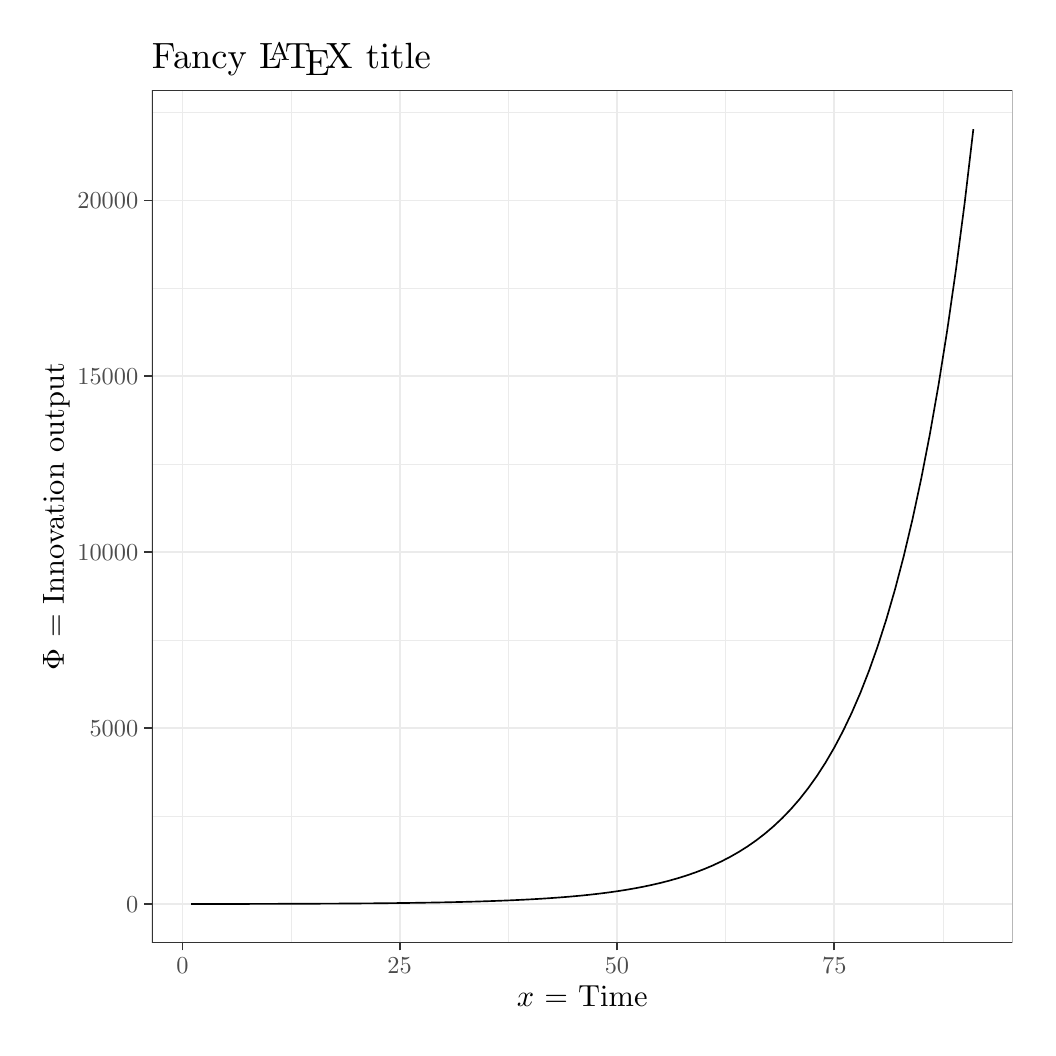
\begin{tikzpicture}[x=1pt,y=1pt]
\definecolor{fillColor}{RGB}{255,255,255}
\path[use as bounding box,fill=fillColor,fill opacity=0.00] (0,0) rectangle (361.35,361.35);
\begin{scope}
\path[clip] (  0.00,  0.00) rectangle (361.35,361.35);
\definecolor{drawColor}{RGB}{255,255,255}
\definecolor{fillColor}{RGB}{255,255,255}

\path[draw=drawColor,line width= 0.6pt,line join=round,line cap=round,fill=fillColor] (  0.00,  0.00) rectangle (361.35,361.35);
\end{scope}
\begin{scope}
\path[clip] ( 44.91, 30.69) rectangle (355.85,338.69);
\definecolor{fillColor}{RGB}{255,255,255}

\path[fill=fillColor] ( 44.91, 30.69) rectangle (355.85,338.69);
\definecolor{drawColor}{gray}{0.92}

\path[draw=drawColor,line width= 0.3pt,line join=round] ( 44.91, 76.44) --
	(355.85, 76.44);

\path[draw=drawColor,line width= 0.3pt,line join=round] ( 44.91,140.01) --
	(355.85,140.01);

\path[draw=drawColor,line width= 0.3pt,line join=round] ( 44.91,203.57) --
	(355.85,203.57);

\path[draw=drawColor,line width= 0.3pt,line join=round] ( 44.91,267.14) --
	(355.85,267.14);

\path[draw=drawColor,line width= 0.3pt,line join=round] ( 44.91,330.71) --
	(355.85,330.71);

\path[draw=drawColor,line width= 0.3pt,line join=round] ( 95.16, 30.69) --
	( 95.16,338.69);

\path[draw=drawColor,line width= 0.3pt,line join=round] (173.68, 30.69) --
	(173.68,338.69);

\path[draw=drawColor,line width= 0.3pt,line join=round] (252.20, 30.69) --
	(252.20,338.69);

\path[draw=drawColor,line width= 0.3pt,line join=round] (330.72, 30.69) --
	(330.72,338.69);

\path[draw=drawColor,line width= 0.6pt,line join=round] ( 44.91, 44.65) --
	(355.85, 44.65);

\path[draw=drawColor,line width= 0.6pt,line join=round] ( 44.91,108.22) --
	(355.85,108.22);

\path[draw=drawColor,line width= 0.6pt,line join=round] ( 44.91,171.79) --
	(355.85,171.79);

\path[draw=drawColor,line width= 0.6pt,line join=round] ( 44.91,235.36) --
	(355.85,235.36);

\path[draw=drawColor,line width= 0.6pt,line join=round] ( 44.91,298.93) --
	(355.85,298.93);

\path[draw=drawColor,line width= 0.6pt,line join=round] ( 55.90, 30.69) --
	( 55.90,338.69);

\path[draw=drawColor,line width= 0.6pt,line join=round] (134.42, 30.69) --
	(134.42,338.69);

\path[draw=drawColor,line width= 0.6pt,line join=round] (212.94, 30.69) --
	(212.94,338.69);

\path[draw=drawColor,line width= 0.6pt,line join=round] (291.46, 30.69) --
	(291.46,338.69);
\definecolor{drawColor}{RGB}{0,0,0}

\path[draw=drawColor,line width= 0.6pt,line join=round] ( 59.04, 44.69) --
	( 62.18, 44.69) --
	( 65.32, 44.69) --
	( 68.47, 44.70) --
	( 71.61, 44.70) --
	( 74.75, 44.71) --
	( 77.89, 44.71) --
	( 81.03, 44.72) --
	( 84.17, 44.73) --
	( 87.31, 44.74) --
	( 90.45, 44.75) --
	( 93.59, 44.76) --
	( 96.73, 44.77) --
	( 99.87, 44.78) --
	(103.01, 44.79) --
	(106.16, 44.81) --
	(109.30, 44.82) --
	(112.44, 44.84) --
	(115.58, 44.86) --
	(118.72, 44.88) --
	(121.86, 44.91) --
	(125.00, 44.93) --
	(128.14, 44.96) --
	(131.28, 45.00) --
	(134.42, 45.03) --
	(137.56, 45.07) --
	(140.70, 45.12) --
	(143.84, 45.17) --
	(146.99, 45.22) --
	(150.13, 45.28) --
	(153.27, 45.35) --
	(156.41, 45.42) --
	(159.55, 45.50) --
	(162.69, 45.59) --
	(165.83, 45.69) --
	(168.97, 45.80) --
	(172.11, 45.92) --
	(175.25, 46.05) --
	(178.39, 46.20) --
	(181.53, 46.36) --
	(184.68, 46.54) --
	(187.82, 46.74) --
	(190.96, 46.96) --
	(194.10, 47.20) --
	(197.24, 47.47) --
	(200.38, 47.76) --
	(203.52, 48.09) --
	(206.66, 48.45) --
	(209.80, 48.85) --
	(212.94, 49.29) --
	(216.08, 49.78) --
	(219.22, 50.32) --
	(222.37, 50.92) --
	(225.51, 51.58) --
	(228.65, 52.30) --
	(231.79, 53.11) --
	(234.93, 54.00) --
	(238.07, 54.98) --
	(241.21, 56.07) --
	(244.35, 57.27) --
	(247.49, 58.59) --
	(250.63, 60.06) --
	(253.77, 61.68) --
	(256.91, 63.47) --
	(260.06, 65.45) --
	(263.20, 67.64) --
	(266.34, 70.06) --
	(269.48, 72.73) --
	(272.62, 75.68) --
	(275.76, 78.94) --
	(278.90, 82.55) --
	(282.04, 86.54) --
	(285.18, 90.94) --
	(288.32, 95.81) --
	(291.46,101.19) --
	(294.60,107.14) --
	(297.74,113.71) --
	(300.89,120.97) --
	(304.03,129.00) --
	(307.17,137.87) --
	(310.31,147.67) --
	(313.45,158.51) --
	(316.59,170.48) --
	(319.73,183.72) --
	(322.87,198.34) --
	(326.01,214.50) --
	(329.15,232.37) --
	(332.29,252.11) --
	(335.43,273.93) --
	(338.58,298.04) --
	(341.72,324.69);
\definecolor{drawColor}{gray}{0.20}

\path[draw=drawColor,line width= 0.6pt,line join=round,line cap=round] ( 44.91, 30.69) rectangle (355.85,338.69);
\end{scope}
\begin{scope}
\path[clip] (  0.00,  0.00) rectangle (361.35,361.35);
\definecolor{drawColor}{gray}{0.30}

\node[text=drawColor,anchor=base east,inner sep=0pt, outer sep=0pt, scale=  0.88] at ( 39.96, 41.62) {0};

\node[text=drawColor,anchor=base east,inner sep=0pt, outer sep=0pt, scale=  0.88] at ( 39.96,105.19) {5000};

\node[text=drawColor,anchor=base east,inner sep=0pt, outer sep=0pt, scale=  0.88] at ( 39.96,168.76) {10000};

\node[text=drawColor,anchor=base east,inner sep=0pt, outer sep=0pt, scale=  0.88] at ( 39.96,232.33) {15000};

\node[text=drawColor,anchor=base east,inner sep=0pt, outer sep=0pt, scale=  0.88] at ( 39.96,295.90) {20000};
\end{scope}
\begin{scope}
\path[clip] (  0.00,  0.00) rectangle (361.35,361.35);
\definecolor{drawColor}{gray}{0.20}

\path[draw=drawColor,line width= 0.6pt,line join=round] ( 42.16, 44.65) --
	( 44.91, 44.65);

\path[draw=drawColor,line width= 0.6pt,line join=round] ( 42.16,108.22) --
	( 44.91,108.22);

\path[draw=drawColor,line width= 0.6pt,line join=round] ( 42.16,171.79) --
	( 44.91,171.79);

\path[draw=drawColor,line width= 0.6pt,line join=round] ( 42.16,235.36) --
	( 44.91,235.36);

\path[draw=drawColor,line width= 0.6pt,line join=round] ( 42.16,298.93) --
	( 44.91,298.93);
\end{scope}
\begin{scope}
\path[clip] (  0.00,  0.00) rectangle (361.35,361.35);
\definecolor{drawColor}{gray}{0.20}

\path[draw=drawColor,line width= 0.6pt,line join=round] ( 55.90, 27.94) --
	( 55.90, 30.69);

\path[draw=drawColor,line width= 0.6pt,line join=round] (134.42, 27.94) --
	(134.42, 30.69);

\path[draw=drawColor,line width= 0.6pt,line join=round] (212.94, 27.94) --
	(212.94, 30.69);

\path[draw=drawColor,line width= 0.6pt,line join=round] (291.46, 27.94) --
	(291.46, 30.69);
\end{scope}
\begin{scope}
\path[clip] (  0.00,  0.00) rectangle (361.35,361.35);
\definecolor{drawColor}{gray}{0.30}

\node[text=drawColor,anchor=base,inner sep=0pt, outer sep=0pt, scale=  0.88] at ( 55.90, 19.68) {0};

\node[text=drawColor,anchor=base,inner sep=0pt, outer sep=0pt, scale=  0.88] at (134.42, 19.68) {25};

\node[text=drawColor,anchor=base,inner sep=0pt, outer sep=0pt, scale=  0.88] at (212.94, 19.68) {50};

\node[text=drawColor,anchor=base,inner sep=0pt, outer sep=0pt, scale=  0.88] at (291.46, 19.68) {75};
\end{scope}
\begin{scope}
\path[clip] (  0.00,  0.00) rectangle (361.35,361.35);
\definecolor{drawColor}{RGB}{0,0,0}

\node[text=drawColor,anchor=base,inner sep=0pt, outer sep=0pt, scale=  1.10] at (200.38,  7.64) {$x$ = Time};
\end{scope}
\begin{scope}
\path[clip] (  0.00,  0.00) rectangle (361.35,361.35);
\definecolor{drawColor}{RGB}{0,0,0}

\node[text=drawColor,rotate= 90.00,anchor=base,inner sep=0pt, outer sep=0pt, scale=  1.10] at ( 13.08,184.69) {$\Phi$ = Innovation output};
\end{scope}
\begin{scope}
\path[clip] (  0.00,  0.00) rectangle (361.35,361.35);
\definecolor{drawColor}{RGB}{0,0,0}

\node[text=drawColor,anchor=base west,inner sep=0pt, outer sep=0pt, scale=  1.32] at ( 44.91,346.76) {Fancy \LaTeX  \hspace{0.01cm} title};
\end{scope}
\end{tikzpicture}
